
\documentclass{report}
\usepackage[T1]{fontenc} % Fontes T1
\usepackage[utf8]{inputenc} % Input UTF8
\usepackage[nottoc]{tocbibind}
\usepackage{csquotes}
\usepackage[portuguese]{babel} %Usar língua portuguesa
\usepackage{blindtext} % Gerar texto automaticamentez	
\usepackage[printonlyused]{acronym}
\usepackage{hyperref} % para autoref
\usepackage{graphicx}



\begin{document}
%%
% Definições
%

\def\titulo{Trabalho de aprofundamento AP2}
\def\data{9 de Abril de 2019}
\def\autores{André Patacas, Gil Teixeira}
\def\autorescontactos{(93357) andrepatacas@ua.pt, (88194) gilteixeira@ua.pt}
\def\departamento{DETI}
\def\logotipo{ua.pdf}
%
%%%%%% CAPA %%%%%%
%
\begin{titlepage}

\begin{center}
%
\vspace*{50mm}
%
{\Huge \titulo}\\ 
%
\vspace{10mm}
%
{\LARGE \autores}\\ 
%
\vspace{30mm}
%
\begin{figure}[h]
\center
\includegraphics{\logotipo}
\end{figure}
%
\vspace{30mm}
\end{center}
%
\begin{flushright}

\end{flushright}
\end{titlepage}

%%  Página de Título %%
\title{%
{\Huge\textbf{Aplicação para o cálculo de Largura de Banda e de latência}}\\
{\Large \departamento}
}
%
\author{%
    \autores \\
    \autorescontactos 
}

%
\date{\data}
%
\maketitle

\pagenumbering{roman}





\tableofcontents
% \listoftables     % descomentar se necessário
% \listoffigures    % descomentar se necessário


%%%%%%%%%%%%%%%%%%%%%%%%%%%%%%%
\clearpage
\pagenumbering{arabic}

%%%%%%%%%%%%%%%%%%%%%%%%%%%%%%%%
%%%%%% RESUMO %%%%%%
\begin{abstract}
Este relatório serve para descrever uma ferramenta desenvolvida para calcular a largura de banda e a latência da máquina onde a aplicação se encontra a correr. Calculam-se estest valores para um determinado servidor ou para um conjunto, de cardinalidade especificável, de servidores de um país, também especificável. No final a aplicação cria um relatõrio, em csv, e assina-o com a chave privada fornecida por um ficheiro à parte pelo utilizador.

\end{abstract}


\chapter{Introdução}
\label{chap.introducao}

A aplicação foi desenvolvida em python3 no âmbito da disciplina de Laboratórios de Informática, no ano letivo 2018/2019. A adicionar às especificações básicas pedidas, segundo o guião sobre regras do segundo trabalho de aprofundamento, construi-se ainda suporte para pydocs para haver uma explicação mais detalhada sobre cada método e classe no nosso projeto. O programa foi escrito com base em test driven development  (\autoref{chap.metodologia}) e, como tal, os testes unitários e funcionais foram criados primeiro, seguidos por um esqueleto do programa e finalmente por vários updates a ambos ({chap.resultados}) para chegar ao estado em que a aplicação se encontra de momento (\autoref{chap.analise}). Finalmente são tiradas as conclusões sobre os aspetos positivos e, potencialmente, negativos desta solução em concreto (\autoref{chap.conclusao})


\chapter{Metodologia}
\label{chap.metodologia}

\begin{enumerate}
	\item Criar o esqueleto do programa que é agora o inicializador da classe (labi02) se esta for chamada diretamente;
	\item Criar o ficheiro test\_labi\_02 como um teste que, apenas se a construção da aplicação for robusta e exatamente como especificada, passa.
	\item Criar o programa labi\_02 e definir as funções com os argumentos de entrada e cada uma com uma descrição detalhada, disponivel nos pydocs, dos aspetos funcionais de cada função.
	\item Ajustar os métodos de forma a que a aplicação passa todos os testes impostos no teste criado.
	\item Testar o programa manualmente e/ou com testes funcionais.
	\item Corrigir eventuais erros.
	\item Iterar o processo de debugging e correção de erros.
\end{enumerate}


\chapter{Aplicação de Speed Test}
\label{chap.Aplicação de Speed Test}
\section{client.py}
\label{sec.client}
\hspace{5mm}Esta é a aplicação que foi desenvolvida e que pode ser utilizada diretamente de acordo com o usage demonstrado ao correr a aplicação sem argumentos. Toda a descrição feita neste relatório remete na mesma para a documentação, esta criada a quando do desenvolvimento da aplicação.

\subsection{main}
Este método é utilizado quando a app é chamada como classe principal (\textit{main}).
Inicialmente chama o método validate (\autoref{subsec.validate}), seguido de run\_tests (\autoref{subsec.runt}), depois o report \autoref{subsec.report} com o resultado da anterior e finalmente assina esse relatório com o método create\_signed\_document (\autoref{subsec.signDoc}).

\subsection{calc\_download()}
\label{subsec.download}
Cálculo da largura de banda.\\
Este método pede, inicialmente, para fazer um download de 100 megabytes ao target server dentro de 10 segundos. Depois verifica que não há mais data para ser recebida do \textit{target\_server} e finalmente calcula o time download 1mb que a máquina demora a fazer download de 1 megabyte.\\ 
\textbf{Argumentos}: \textit{target\_server}(dicionário com informação sobre o target server). 
\textbf{Retorna}: (float) $1/\textit{time\_download\_1mb}$

\subsection{calc\_latency()}
\label{subsec.latency}
\hspace{5mm}Cálculo da latência.\\ 
Este método tenta trocar dez comandos PING-PONG com o targe-server e calcula o tempo médio em milisegundos entre estas trocas.\\
\hspace{5mm}\textbf{Argumentos}: target server (dicionário com informação sobre o target server). 
\hspace{5mm}\textbf{Retorna}:(int) \textit{average\_trade\_time} em ms.

\subsection{country\_test()}
\label{subsec.countrytest}
\hspace{5mm}Este método serve para calcular a largura de banda e latency da conexção a um servidor random do país passado como argumento.\\ 
\hspace{5mm}\textbf{Argumentos}: (str) \textit{target\_country}.\\
\textbf{Retorna}: objeto \textit{SpeedTestResult} com as informações relativas aos resultados do teste.

\subsection{create\_signed\_document}
\label{subsec.signDoc}
\hspace{5mm}Este método gera um \textit{signature file} assinando o \textit{report} com a chave privada no \textit{key\_path} especificado.\\ 
\hspace{5mm}\textbf{Argumentos}: 
\begin{enumerate}
\item \textit{key\_path} (str): The path to the file that contains the key;
\item \textit{report\_name} (str): Nome do \textit{report} a ser assinado;
\item \textit{signature\_name} (str): Nome do \textit{signature file} que será gerado.	
\end{enumerate}
\textbf{Retorna}: \textit{None}.

\subsection{id\_test()}
\label{subsec.idtest}
\hspace{5mm}Este método serve para calcular a largura de banda e latency da conexão a um servidor com o id passado como argumento.\\ 
\hspace{5mm}\textbf{Argumentos}: (int) \textit{target\_id}.\\
\textbf{Retorna}: objeto \textit{SpeedTestResult} com as informações relativas aos resultados do teste.

\subsection{random\_test()}
\label{subsec.randt}
Este método serve para calcular a largura de banda e latency da conexção a um servidor random.\\ 
\textbf{Argumentos}: \textit{None}.\\
\textbf{Retorna}: objeto \textit{SpeedTestResult} com as informações relativas aos resultados do teste.

\subsection{report()}
\label{subsec.report}
Este método vai gerar um \textit{test\_report} basiado numa lista de objetos \textit{SpeedTestResult} passados como argumentos.\\ 
\textbf{Argumentos}:
\begin{enumerate}
\item List[objeto \textit{SpeedTestResult}];
\item \textit{report\_name} (str) - nome do ficheiro a ser gerado.
\end{enumerate}
\textbf{Retorna}: \textit{None}. O ficheiro \textit{test\_report} será gerado

\subsection{run\_tests()}
\label{subsec.runt}
Este método serve para calcular a largura de banda e latency da conexção a um \textit{num} de servidores num país ou a um server com o id passado por argumento.\\
Nota: se o terceiro argumento for um id a função realizará \textit{num} testes a esses servidor, se for um país fará \textit{num} testes usando a função \autoref{subsec.countrytest} e se não foi passado terceiro argumento realiza um teste random (\autoref{subsec.randt}).\\
\textbf{Argumentos}: 
\begin{enumerate}
\item \textit{inteval}: intervalo de tempo entre cada teste realizado;
\item \textit{num}: número de testes a realizar;
\item \textit{id\_or\_country}: país (str) ou id (int) de um server;
\item \textit{option}: -v se pretender correr a aplicação em modo \textit{verbose}.
\end{enumerate}
\textbf{Retorna}: objeto \textit{SpeedTestResult} com as informações relativas aos resultados do teste.

\subsection{validate()}
\label{subsec.validate}
Este método trata da validação dos argumentos passados pela variávle sys.argv.\\ 
\textbf{Argumentos}: \textit{None}.\\
\textbf{Retorna}: \textit{None}.

\subsection{usage()}
\label{subsec.usage}
Este método imprime a mensagem de erro passada como argumento e imprime a ajuda para utilização da aplicação. No campo \textit{option} pode usar \textit{-v} para entrar em modo verbose.\\ 
\textbf{Argumentos}: \textit{message} (str).\\
\textbf{Retorna}: \textit{None}.

\subsection{log()}
\label{subsec:log}
Este método imprime a mensagem de passada como argumento com a cor passada como argumento.\\ 
\textbf{Argumentos}: 
\begin{enumerate}
\item \textit{message} (str);
\item \textit{colour} (str).
\end{enumerate}
\textbf{Retorna}: \textit{None}.

\subsection{log\_error()}
Este método chama \autoref{subsec:log} com a mensagem igual à passada como argumento mas com cor vermelho.\\ 
\textbf{Argumentos}:
\textit{message} (str).\\
\textbf{Retorna}: \textit{None}.

\subsection{log\_warning()}
Este método chama \autoref{subsec:log} com a mensagem igual à passada como argumento mas com cor amarela.\\ 
\textbf{Argumentos}:
\textit{message} (str).\\
\textbf{Retorna}: \textit{None}.

\subsection{log\_verbose()}
Este método chama \autoref{subsec:log} com a mensagem igual à passada como argumento mas com cor verde se o modo \textit{verbose} estiver ativado.\\ 
\textbf{Argumentos}:
\textit{message} (str).\\
\textbf{Retorna}: \textit{None}.

\subsection{load\_server()}
Este método lê o ficheiro \textit{"servers.json"} e cria um dicionário global com a lista de servidores.\\
\textbf{Argumentos}:
\textit{None}.\\
\textbf{Retorna}: \textit{None}.

\section{test\_client}
Este programa é constituida por métodos que são testes unitários aos da aplicação principal (\autoref{sec.client}). Lista \{\textit{teste unitário : método (da \autoref{sec.client})}\}:
\begin{enumerate}
\item test\_calc\_download() : \autoref{subsec.download};
\item test\_calc\_latency(): \autoref{subsec.latency};
\item test\_country\_test(): \autoref{subsec.countrytest};
\item test\_create\_signed\_document(): \autoref{subsec.signDoc};
\item test\_id\_test(): \autoref{subsec.idtest};
\item test\_random\_test(): \autoref{subsec.randt};
\item test\_report(): \autoref{subsec.report};
\item test\_run\_test(): \autoref{subsec.runt}.
\end{enumerate}

\section{speed\_test\_result}
Este programa serve para criar objetos SpeedTestResult que têm, cada um, as informações respetivas a um teste. Tem apenas um construtor e um método:
\subsection{Construtor}
O construtor da classe cria um objeto com os parametros passados como argumentos:
\textbf{Argumentos}:
\begin{enumerate}
\item \textit{server\_id} (int);
\item \textit{download\_speed} (float);
\item \textit{latency} (int);
\end{enumerate}

\subsection{getObjDict}
Este método devolve um dicionário com os resultados do teste relativo ao objeto.
\textbf{Argumentos}: \textit{None}.\\
\textbf{Retorna}: \textit{testResult} (dict).

\chapter{Exemplo de utilização}
\label{chap:example}
Com exemplo ir-se-á correr a aplicação \autoref{sec.client} com os argumentos:
\begin{enumerate}
\item \textit{interval} = 5 (segundos);
\item \textit{num} = 3 (testes);
\item \textit{id\_or\_country} = Portugal;
\item \textit{option} = -v (\textit{verbose}).
\end{enumerate}
Ao correr a aplicação com estes argumentos, segundo a \autoref{subsec.usage}, vêm os seguintes resultados:\\
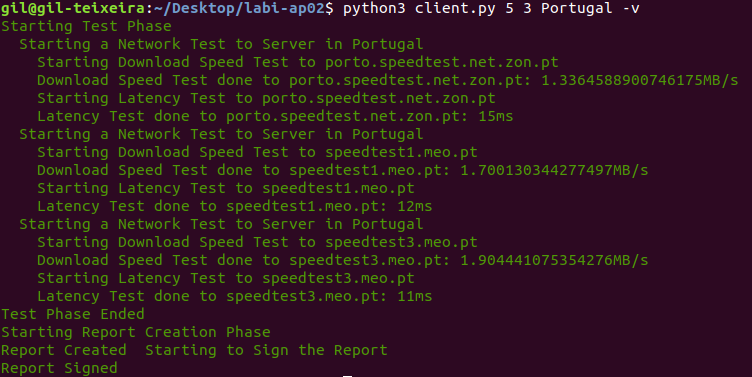
\includegraphics[width=\textwidth]{useExample}
Criando-se dois novos ficheiros na pasta onde está a aplicação:
\begin{itemize}
\item report.sig, contendo uma assinatura do relatório pela chave privada fornecida (\textit{key.priv}).
\item report.csv, um ficheiro \ac{csv} com os resultados dos três testes efetuados:
\end{itemize}
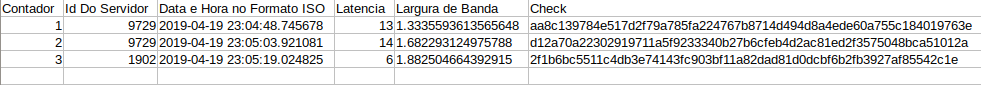
\includegraphics[width=\textwidth]{reportcsv}


\chapter{Análise}
\label{chap:analise}
\chapter{Conclusão}
\label{chap:conclusao}
\chapter*{Acrónimos}
\begin{acronym}
\acro{ua}[UA]{Universidade de Aveiro}
\acro{miect}[MIECT]{Mestrado Integrado em Engenharia de Computadores e Telemática}
\acro{guiaomini}[Mini-projeto]{Universidade de Aveiro
		Dep. de Electrónica, Telecomunicações e Informática
		Laboratório de Sistemas Digitais}
\acro{csv}[CSV]{Comma-separated values}
\end{acronym}
%%%%%%%%%%%%%%%%%%%%%%%%%%%%%%%%%



%%%%%%%%%%%%%%%%%%%%%%%%%%%%%%%%%


\end{document}
